\documentclass[]{amsart}
\setlength{\marginparwidth}{0.5in}
\usepackage{amsmath,amssymb,amsthm,mathtools,booktabs,array,tikz,pifont,comment,graphicx}
\usepackage[author-year]{amsrefs}
\input FJHDef.tex

%Requires ApproxUnivariate.tex, univariate_integration.tex, foolbwquadexample.eps 

\DeclareMathOperator{\INT}{INT}
\DeclareMathOperator{\lin}{lin}
\DeclareMathOperator{\up}{up}
\DeclareMathOperator{\lo}{lo}
\DeclareMathOperator{\fix}{non}
\DeclareMathOperator{\err}{err}
\DeclareMathOperator{\maxcost}{maxcost}
\DeclareMathOperator{\mincost}{mincost}
\newcommand{\herr}{\widehat{\err}}

\newtheorem{theorem}{Theorem}
\newtheorem{prop}[theorem]{Proposition}
\newtheorem{lem}{Lemma}
\newtheorem{cor}{Corollary}
\theoremstyle{definition}
\newtheorem{algo}{Algorithm}
\newtheorem{condit}{Condition}
%\newtheorem{assump}{Assumption}
\theoremstyle{remark}
\newtheorem{rem}{Remark}
\newcommand{\Fnorm}[1]{\abs{#1}_{\cf}}
\newcommand{\Gnorm}[1]{\abs{#1}_{\cg}}
\newcommand{\flin}{f_{\text{\rm{lin}}}}


\begin{document}

\title{Reliable Automatic Quadrature for Cones of Integrands}
\author{Fred J. Hickernell}
\author{Martha Razo}
\author{Sunny Yun}
\maketitle 


\begin{abstract} Hi
\end{abstract}


\section{Introduction} 

Automatic numerical algorithms for univariate integration appear in many widely used software packages, such as MATLAB \ycite{MAT8.1}, Mathematica \ycite{Mat9a}, NAG \ycite{NAG23}, and R \ycite{R2512}.  Automatic algorithms determine adaptively where and how much to sample the integrand by estimating the algorithm error from the sampled function values.  Unfortunately, such error estimation methods are unreliable, as pointed out by James Lyness \ycite{Lyn83}.
We now know that Lyness's objections can be overcome by employing a new paradigm for error estimation for cones of integrands.  The discussion here illustrates with greater detail the more general setting in \ocite{HicEtal14b}.

Soon after a calculus student first learns about integration, she learns that the integrals of many elementary functions are \emph{not} themselves elementary functions.  An important example is the standard normal probability density function, $\phi: x \mapsto \me^{-x^2}/\sqrt{2 \pi}$.  Since the antiderivative of $\phi$ cannot be expressed in terms of elementary functions, we need tables in textbooks and special functions in calculators to provide the values of the standard normal distribution function $\Phi : x \mapsto \int_{-\infty}^x \phi(t) \, \dif t$. By contrast, the derivaties of elementary functions are elementary functions.  

\subsection{The Trapezoidal Rule}
Students need to know that the lack of an analytic answer does not mean that no answer exists, so calculus students are often introduced to numerical integration (quadrature) methods such as the trapezoidal rule, $T_n$:
\begin{equation}
\int_0^1 f(x) \, \dif x \approx T_n(f) := \frac{1}{2n} \left [ f(0) + 2 f(1/n) + \cdots + 2 f(1-1/n) + f(1) \right].
\end{equation}
It is then natural to ask, ``How large should the number of trapezoids, $n$, be so that the absolute error of $T_n(f)$ does not exceed a tolerance $\varepsilon$?''  There is an error bound of the form
\begin{equation} \label{traperrbd}
\err(f,n) := \abs{\int_0^1 f(x) \, \dif x - T_n(f)} \le \frac{V(f')}{8n^2}, \qquad n \in \naturals = \{1, 2, \ldots \}. 
\end{equation}
Here, $V(\cdot)$ denotes the total variation, which is defined as
\begin{equation} \label{vardef}
V(f) := \sup_{\substack{n \in \naturals\\ 0 = x_0 < x_1 < \cdots < x_{n} =1}} \sum_{i=1}^n \abs{f(x_i)-f(x_{i-1})}.
\end{equation}
The norm $V(\cdot)$ is related to $\cl_p$-norms as follows:
\begin{equation}
V(f)= \norm[1]{f'} \text{ if } \norm[1]{f'}< \infty, \qquad 
\norm[p]{f}:= \begin{cases} \displaystyle \left[\int_0^1 \abs{f(x)}^p \, \dif x \right]^{1/p}, & 1 \le p < \infty,\\[1ex]
\displaystyle  \sup_{0 \le x \le 1} \abs{f'(x)}, & p=\infty.
\end{cases}
\end{equation}
Error bounds resembling \eqref{traperrbd} exist in terms of $\cl_p$-norms of $f''$ but with different leading constants.  

If $f$ has a simple form, one might be able to derive an upper bound, $M_1$, on this norm, i.e., $V(f') \le M_1$.  In this case choosing any $n \ge \sqrt{M_1/(8\varepsilon)}$ ensures that the error tolerance is met. For example, for $\phi$ defined above, $V(f')=1/\sqrt{2 \pi \me}$, and so one may choose any $n \ge 1/\sqrt{8\sqrt{2 \pi \me} \, \varepsilon}$,
\begin{comment}
\begin{equation}
\err(f,n) = \abs{\int_0^1 f(x) \, \dif x - T_n(f)} \le \frac{\norm[1]{f''}}{8n^2}, \qquad 
\norm[p]{f}:= \left[\int_0^1 \abs{f(x)}^p \, \dif x \right]^{1/p}.
\end{equation}
Similar error bounds exist in terms of other $\cl_p$-norms of $f''$.  If $f$ has a simple form, one might be able to derive an upper bound, $M_1$, on this norm, i.e., $\norm[1]{f''} \le M_2$.  In this case choosing any $n \ge \sqrt{M_2/(8\varepsilon)}$ ensures that the error tolerance is met. For example, for $\phi$ defined above, $\norm[1]{f''}=1/\sqrt{2 \pi \me}$, and so one may choose any $n \ge 1/\sqrt{8\sqrt{2 \pi \me} \, \varepsilon}$.
\end{comment}

\section{The Flaws in the Prevalent Data-Based Error Estimate}
It is often impractical to bound $V(f')$ analytically because the formula for $f$ is not given explictly  or because it is too complicated.  A more widely applicable quadrature method would reliably estimate the error based solely on the function values, $f(x_i)$, and determine the sample size appropriately.  Numerical methods texts, such as \ocite{BurFai10}*{p.\ 223--224}, \ocite{CheKin12a}*{p.\ 233}, and  \ocite{Sau12a}*{p.\ 270}, advise the readers to estimate the error by comparing two trapezoidal rules with different numbers of trapezoids, specifically,
\begin{equation}\label{baderr}
\herr(f,n) = \frac{T_n(f) - T_{n/2}(f)}{3}, \qquad \frac n2 \in \naturals.
\end{equation}
One may then compute $\herr(f,2^j)$ for $j=1, 2, \ldots$ and stop when $\herr(f,2^j) \le \varepsilon$.  By doubling the number of trapezoids for each iteration, the data from the previous iterations can be reused.  

Unfortunately, it is easy to construct integrands, $f$, such that this error estimate fails completely, e.g.,
\begin{equation} \label{failcond}
\int_0^1 f(x) \, \dif x =  1, \quad T_{n}(f)=T_{n/2}(f) = -1, \quad \err(f,n)=2 \ne 0 = \herr(f,n).
\end{equation}
Figure \ref{spikeflukefig} shows two examples satisfying these conditions. These two examples illustrate the two ways in which the error estimate $\herr(\cdot)$, and any automatic quadrature algorithm base on it, can fail.  One way is ultimately unavoidable but ought to be quantifiable.  The other way is inexcusable, but is prevalent in widely used automatic numerical quadrature.

\begin{figure}
\centering 
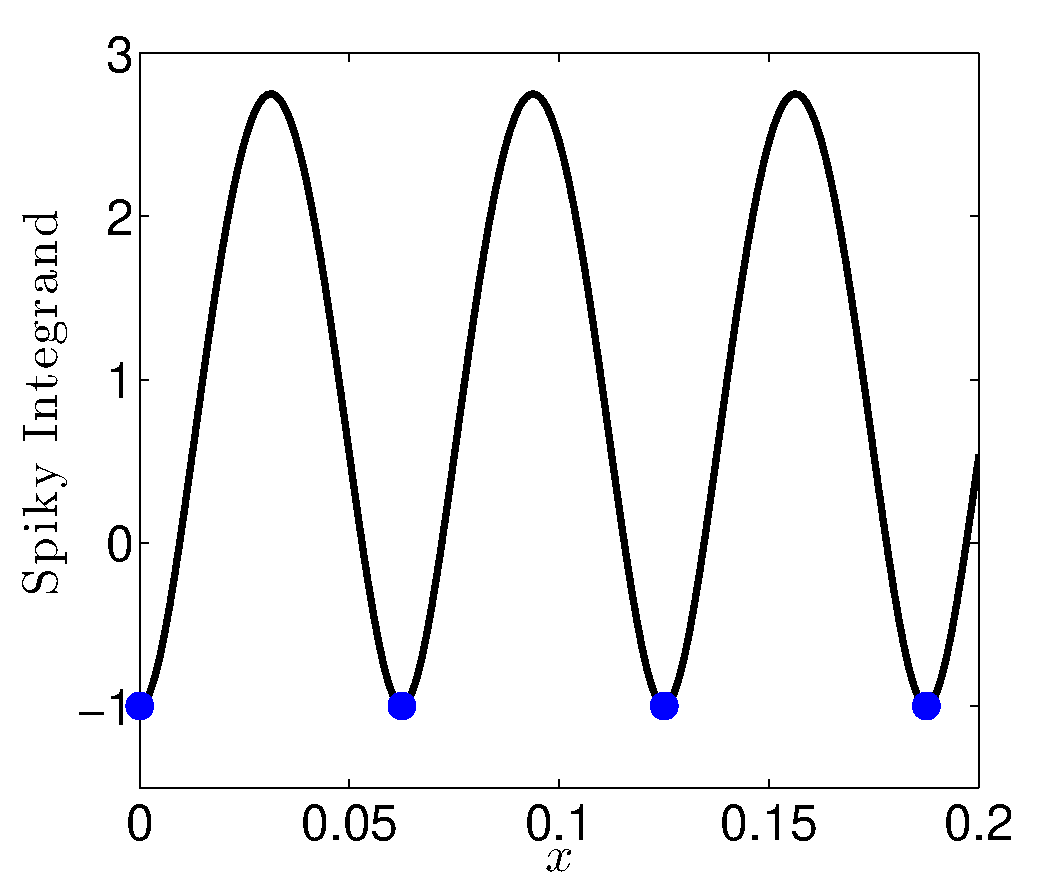
\includegraphics[width=6cm]{SpikyIntegFigcolor.eps} \quad
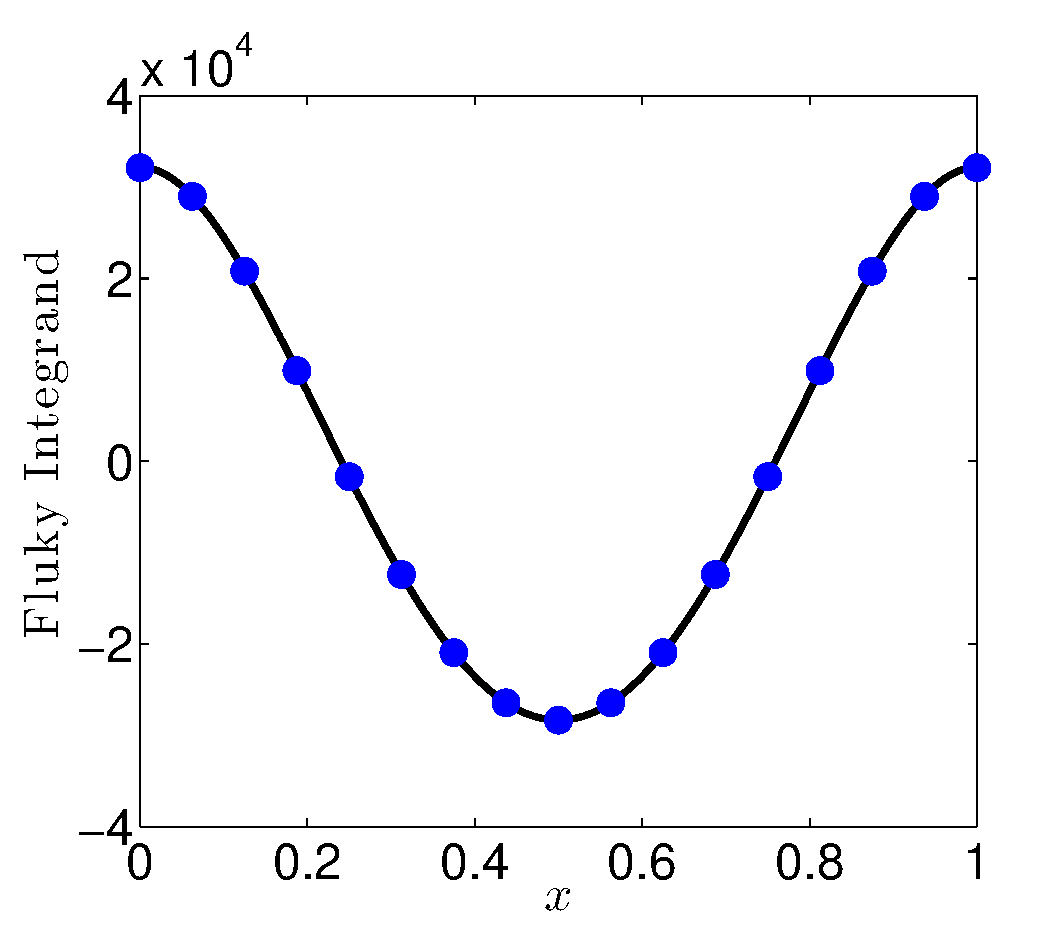
\includegraphics[width=6cm]{FlukyIntegFigcolor.eps}
\caption{Examples of a spiky integrand (left) and a fluky integrand (right), which satisfy \eqref{failcond} for $n=32$. \label{spikeflukefig}}
\end{figure}

\subsection{Spiky Integrands} \emph{Any} quadrature algorithm that depends on just function values to estimate error will be fooled by a spiky integrands.  Suppose that the quadrature algorithm samples the integrand at a seqeunce of points, $\xi_1, \xi_2, \ldots$, and suppose that $f(\xi_i)$ is the same value for all $\xi_i$.  Here the algorithm may even be adaptive, meaning that $\xi_{i+1}$ may depend on $(\xi_1, f(\xi_1)), \ldots, (\xi_i, f(\xi_i))$.  Eventually the algorithm stops at $n$ points.  Under mild conditions on the set of integrands of interest the best estimate of the integral is that constant. 

Figure \ref{spikeflukefig} (left) plots a spiky integrand that is defined in terms of the quartic Bernoulli polynomial:
\begin{equation} \label{spiky}
f_{\text{spiky}}(x;n) = 1 + 60 B_4(\bbl nx \bbr), \qquad n \in \naturals, \quad \bbl x \bbr := x \bmod 1.
\end{equation}
The Bernoulli polynomials are described by \ocite{AbrSte64}*{Chap.\ 23, \url{http://dlmf.nist.gov/24}}.  The first six are defined as follows 
\begin{subequations} \label{Bernoulli}
\begin{gather} 
B_0(x) = 1, \qquad B_1(x) = x-1/2,  \qquad 
B_2(x)=1/6 - x(1-x), \\ 
B_3(x) = \frac{1}{2} x(1-x)(1-2x), \qquad B_4(x) = -1/30 + [x(1-x)]^2, \\
B_5(x) = \frac{1}{6} x(1-x)(1-2x)(1 + 3 x - 3 x^2).
\end{gather}
\end{subequations}
The integrand $f_{\text{spiky}}(\cdot;n)$ satisfies \eqref{failcond} for even $n$ and has 
\begin{itemize}
\item $n+1$ local minima of $-1$ at $x=0, 1/n, \ldots, 1$, and
\item $n$ local maxima of $11/4$ at $x=1/(2n), 3/(2n), \ldots, 1-1/(2n)$.
\end{itemize}

The problem of integrating spiky functions never goes away, but it should be quantifiable.  An algorithm ought to integrate functions accurately, provided that they have spikes no thinner than say, $\delta$.  Moreover, the algorithm should be tunable so that the user can specifiy $\delta$.  We describe such an algorithm in Section \ref{newalgosec}, along with a precise definition of spike width.

\subsection{Fluky Integrands} 

Thirty years ago James Lyness \ycite{Lyn83}*{p.\ 69} made the following observation in his SIAM Review article, \emph{When Not to Use an Automatic Quadrature Routine}:
\begin{quote}
While prepared to take the risk of being misled by chance alignment of zeros in the integrand function, or by narrow peaks which are ``missed,'' the user may wish to be reassured that for ``reasonable'' integrand functions which do not have these characteristics all will be well. It is the purpose of the rest of this section to demonstrate by example that he cannot be reassured on this point. In fact the routine is likely to be unreliable in a significant proportion of the problems it faces (say $1$ to $5\%$) and there is no way of predicting in a straightforward way in which of any set of apparently reasonable problems this will happen.
\end{quote}
Lyness went on to describe how to construct, what we would call a fluky integrand.  

Figure \ref{spikeflukefig} (right) plots a fluky integrand, which is defined in terms of the quadratic and quartic Bernoulli polynomials:
\begin{equation} \label{fluky}
f_{\text{fluky}}(x;n) = 1 - 15 n^2 [B_2(x) + n^2 B_4(x)], \qquad n \in \naturals.
\end{equation}
The integrand $f_{\text{fluky}}(\cdot;n)$ satisfies \eqref{failcond} for even $n$ and has only 
\begin{itemize}
\item $1$ local minimum of $(16 + 20 n^2 - 7 n^4)/16$ at $x=1/2$, and
\item $2$ local maxima of $(19 - 10 n^2 + 2 n^4)/4$ at $x=(1 \pm \sqrt{1 -2/n^2})/2$.
\end{itemize}
Integrands like this one are termed by us as fluky because their construction is rather delicate.  They satisfy conditions \eqref{failcond} without a large number of local optima.  To illustrate this delicacy, note that removing either the $B_2$ or the $B_4$ term does not affect the value of the integral but does cause the trapezoidal rule estimates of the integral to vary significantly for $n$ and $n/2$ trapezoids.

The failure of the error estimate in \eqref{baderr} for $f_{\text{fluky}}(\cdot;n)$ seems avoidable. For even moderate $n$, the sampled function values, $\bigl(f_{\text{fluky}}(i/n;n)\bigr)_{i=1}^{n}$, are spread across a large range.  This suggests that true error, $\err(f_{\text{fluky}}(\cdot;n),n)$, might be substantial, and far from the error estimate, $\herr(f_{\text{fluky}}(\cdot;n),n)=0$.  In Section \ref{newalgosec} we transform this intuition into a better method for estimating the error of the trapezoidal rule.

\subsection{Necessary Conditions for Failure of the Error Estimate} 
Integrands that satisfy \eqref{failcond} and fool the error estimate in \eqref{baderr} must satisfy certain conditions.  First note that the error bound in \eqref{traperrbd}
\[
V(f') \ge 8n^2 \err(f,n) =  16n^2,
\]
so the total variation of the first derivative must be increasingly large as the number of trapezoids increases.  Moreover, the trapezoidal rule added to the error estimate in \eqref{traperrbd} results in Simpson's rule:
\begin{align*}
S_n(f) &:= T_n(f) + \herr(f,n) = \frac{4T_n(f) - T_{n/2}(f)}{3} \\
& = \frac{1}{3n} \left [ f(0) + 4 f(1/n) + 2 f(2/n) + 4 f(3/n) + \cdots + 4 f(1-1/n) + f(1) \right]
\end{align*}
The error bound of Simpson's rule then serves as an bound on the error of the error estimate:
\begin{equation} \label{Simperrbd}
\abs{\err(f,n) - \herr(f,n)} = \abs{\int_0^1 f(x) \, \dif x - S_n(f)} \le \frac{V(f''')}{???n^4}, \qquad \frac{n}2 \in \naturals. 
\end{equation}
So, integrands satisfying \eqref{failcond} must also satisfy
\[
V(f''') \ge ??n^4 \abs{\err(f,n) - \herr(f,n)} =  ???n^4.
\]
Thus, the total variation of the third derivative must be increase even faster as the number of trapezoids increases.

The derivatives of Bernoulli polynomials are multiples of lower degree Bernoulli polynomials and the integrals of nonconstant Bernoulli polynomials vanish \cite{AbrSte64}*{Chap.\ 23, \url{http://dlmf.nist.gov/24}}:
\[
B'_n(x) = n B_{n-1}(x), \quad \int_0^1 B_{n+1}(x) \, \dif x, \qquad n \in \naturals.
\]
The formula for the derivatives facilitates the computation of the total variation of the spiky and fluky examples above.  For the spiky integrand defined in \eqref{spiky},
\begin{subequations} \label{spikyvariation}
\begin{gather}
f'_{\text{spiky}}(x;n) = 240 n B_3(\bbl nx \bbr), \qquad f''_{\text{spiky}}(x;n) = 720 n^2 B_2(\bbl nx \bbr), \\ f'''_{\text{spiky}}(x;n) = 1440 n^3 B_1(\bbl nx \bbr), \\
V(f_{\text{spiky}}(\cdot;n))= \frac{15n}{2}, \qquad  V(f'_{\text{spiky}}(\cdot;n))= \frac{80n^2}{\sqrt{3}} > 16 n^2, \\
V(f''_{\text{spiky}}(\cdot;n))= 360n^3, \qquad V(f'''_{\text{spiky}}(\cdot;n))= 1440n^4.
\end{gather}
\end{subequations} 
For the fluky integrand defined in \eqref{fluky},
\begin{subequations} \label{spikyvariation}
\begin{gather}
f'_{\text{fluky}}(x;n) = - 30 n^2 [B_1(x) + 2 n^2 B_3(x)], \\ f''_{\text{fluky}}(x;n) = -30 n^2 [1 + 6 n^2 B_2(x)], \qquad f'''_{\text{fluky}}(x;n) = -360 n^4 B_1(x), \\
V(f_{\text{fluky}}(\cdot;n))= \frac{15}{8} (8 - 4 n^2 + n^4),  \\
V(f'_{\text{fluky}}(\cdot;n))= \frac{10 n}{3}  \Bigl[9 n + 2 \sqrt{3(-2 + n^2)^3} \Bigr ]  > 16 n^2, \\
V(f''_{\text{fluky}}(\cdot;n))= 90n^4, \qquad V(f'''_{\text{fluky}}(\cdot;n))= 360n^4.
\end{gather}
\end{subequations}  

Note that the variations of the integrand its derivatives behaves differently for these two examples:
\[
V(f^{(j)}_{\text{spiky}}(\cdot;n)) \asymp n^{j+1}, \quad V(f^{(j)}_{\text{fluky}}(\cdot;n)) \asymp n^{4}, \qquad j=0, \ldots, 3.
\]
For the spiky integrand the asymptotic order of the total variation for large $n$ increases with the order of the derivative while for the fluky integrand it stays the same.

\section{A Guaranteed Quadrature Algorithm} \label{newalgosec}

Now we turn to a new error estimate for numerical integration proposed in 

\section{Acknowledgements}  The authors are grateful for discussions with a number of colleagues. This research is supported in part by grant NSF-DMS-1115392.

\bibliography{FJH22,FJHown22}
\end{document}

